\documentclass{article}
\usepackage[top=1.0in,bottom=1.0in,left=1.0in,right=1.0in]{geometry}
\usepackage{amsmath,amssymb,amsthm,amsfonts}
\usepackage[utf8]{inputenc}
\usepackage{hyperref}
\usepackage{graphicx}

\title{Triptych: logarithmic-sized linkable ring signatures with applications}
\author{Sarang Noether and Brandon Goodell \\ Monero Research Lab \\ \texttt{\{sarang,surae\}.noether@protonmail.com}}
\date{\today}

\newcommand{\G}{\mathbb{G}}
\newcommand{\F}{\mathbb{F}}
\newcommand{\com}{\operatorname{Com}}
\newcommand{\hs}{\mathcal{H}}
\newcommand{\hp}{\mathbb{H}}

\newcommand{\A}{\mathcal{A}}

\newcommand{\sumi}{\sum_{i=0}^{n-1}}
\newcommand{\sumj}{\sum_{j=0}^{m-1}}
\newcommand{\sumk}{\sum_{k=0}^{N-1}}

\newtheorem{theorem}{Theorem}
\theoremstyle{definition}
\newtheorem{definition}{Definition}

\begin{document}

\maketitle


\begin{abstract}
Ring signatures are a common construction used to provide signer ambiguity among a non-interactive set of public keys specified at the time of signing.
Unlike early approaches where signature size is linear in the size of the signer anonymity set, current optimal solutions either require centralized trusted setups or produce signatures logarithmic in size.
However, few also provide linkability, a property used to determine whether the signer of a message has signed any previous message, possibly with restrictions on the anonymity set choice.
Here we introduce Triptych, a family of linkable ring signatures without trusted setup that is based on generalizations of zero-knowledge proofs of knowledge of commitment openings to zero.
We demonstrate applications of Triptych in signer-ambiguous transaction protocols by extending the construction to openings of parallel commitments in independent anonymity sets.
Signatures are logarithmic in the anonymity set size and, while verification complexity is linear, collections of proofs can be efficiently verified in batches.
We show that for anonymity set sizes practical for use in distributed protocols, Triptych offers competitive performance with a straightforward construction.
\end{abstract}


\section{Introduction}
First introduced in \cite{rivest} with respect to RSA groups, ring signatures permit the signing of messages using public key sets not fixed in advance, without the need of a trusted group manager.
Earlier constructions lacked such flexibility, requiring either centralized key setup or the establishment of fixed signing sets.
Later work \cite{bender} established more robust security models for unforgeability and anonymity, capturing realistic threat models where an adversary is permitted to corrupt keys, convince honest signers to include malicious anonymity set members, or obtain signatures in advance.

Since a ring signature has an anonymity set of public keys, one of which is the true signer, the detection of signing by the same key requires an additional property, linkability.
A linkable ring signature \cite{lsag} enables verifiers to determine whether the (unknown) signer of a message has signed other messages.
Such a construction was proposed for election applications, where it is necessary to ensure that votes are anonymous, but voters are permitted to vote only once on a particular issue.
The construction in \cite{lsag}, with a hash-trapdoor structure similar to that of \cite{schnorr}, is of particular interest due to potential flexibility in linking; while its linking is limited to signer-selected but unchanging signer anonymity sets, it permits linking on a per-issue basis.
Additional recent work in \cite{backes} introduces the property of linkable anonymity, using sets of signatures and establishing restrictions on key corruption.
Other related interesting properties like traceability \cite{fs,f} imply stronger capabilities, where an attempt to sign two messages with the same key permits verifiers to identify the signer.

Linkable ring signatures have seen particular applications in signer-ambiguous transaction protocols.
In such an application, transactions are authorized by a ring signature whose signing anonymity set consists of previously-generated transaction outputs.
A signature demonstrates that the signer controls the private key of one such output without revealing which is the signer, and linkability is used to assure verifiers that output has not been used in another signature (signifying a double-spend attempt).

A practical consideration for the use of linkable ring signatures in transaction protocols is how signature size and verification time scale with the size of the anonymity set.
In common applied constructions like \cite{mlsag,clsag}, signature size and verification time scale linearly with the size of the signing ambiguity set; since such signatures are typically included in a public distributed data structure like a blockchain, there is a balance between the size of the anonymity set and the requirements for storage and verification.
Recent protocol work in this area mitigates the size restriction.
For example, in \cite{rct3}, the authors introduce a confidential transaction protocol based on a proving system whose size scales logarithmically with the anonymity set size, and which includes a method for demonstrating amount balance; amount commitment range proving is offloaded to other constructions like \cite{bulletproofs}.
In \cite{omniring}, the authors use a more general proving technique to accomplish a similar goal; however, the protocol offers further size benefits by integrating commitment range proofs into the proof structure directly, taking advantage of the logarithmic proof size.

Other signer-ambiguous transaction protocols not based on linkable ring signatures offer more competitive performance.
For example, protocols like \cite{zcash} produce maximal theoretical signer ambiguity through the use of zero-knowledge Merkle proofs (among others) that offer extremely small proofs with low verification time, but at the cost of a trusted structured setup process that arises from the underlying proving system \cite{groth16}.
Like this work, \cite{lelantus} is a transaction protocol also based on \cite{groth}; however, it is intended to operate on commitments similar to those used in \cite{zerocoin} but with the inclusion of amounts, and has limitations on addressing and sender tracing.


\subsection{Our contribution}
We produce a family of linkable ring signatures, which we call Triptych.
The constructions are a linkable generalization of Groth's one-of-many commitment-to-zero proving system \cite{groth}, with optimizations from Bootle \cite{bootle} applied for improvements to proof size and verification complexity.
In the simplest version of Triptych, the prover shows that it knows the opening of a commitment to zero within a commitment set, and also that it has constructed a linking tag using the same opening, producing a linkable ring signature construction.
We then modify Groth's ring signature definitions to include linkability and a related property, non-frameability.

In an extension of Triptych, we include multiple independent sets of commitments.
Here, the prover proceeds as before to show its knowledge of an opening to a commitment in one set, as well as the construction of the linking tag.
However, the proof also shows that the prover knows an opening of a commitment at the same position in all other sets.
This construction has immediate application; in some signer-ambiguous confidential transaction protocols, transaction inputs are commitments to zero, for which the signer shows it knows the opening.
Each commitment comes equipped with another commitment to the amount of the input; by offsetting these commitments homomorphically and carefully choosing commitment randomness, the prover can show that a particular transaction balances.

We show that Triptych produces signatures with competitive performance to other modern linkable ring signatures for limited anonymity set sizes.
We note that similar constructions also require linear verification time, meaning that the size of anonymity set used in practice is likely to be limited for performance reasons.


\section{Preliminaries}
\subsection{Public parameters}
Let $\G$ be a cyclic group in which the discrete logarithm problem is hard, and let $\F$ be the scalar field of $\G$.
Let $\hs: \{0,1\}^* \to \F$ be a cryptographic hash function.
Let $G$ and $H$ be generators of $\G$ with unknown discrete logarithm relationship.
Let $N = n^m$ be a size parameter, where $n > 1$ and $m > 1$.
Let $\{G_{j,i}\}_{j,i=0}^{m-1,n-1}$ be a set of generators of $\G$ with unknown discrete logarithm relationship to each other, to $G$, and to $H$.
Let $U$ be a generator of $\G$.
Note that all generators may be produced using public randomness; for example, the use of a suitable hash function with domain separation may be appropriate.
All such public parameters are assumed to comprise a global reference string known to all players; in particular, we exclude them from algorithm definitions and Fiat-Shamir transcript hashes for readability.


\subsection{Pedersen commitment}
Let $\com$ be a homomorphic commitment scheme that is perfectly hiding and computationally binding.
In this work, we assume use of the Pedersen commitment scheme: for $x,r \in \F$, define $\com(x,r) \equiv xG + rH$ to be the commitment of the value $x$ with randomness $r$.
This can be trivially extended to support matrix values; for $\{x_{j,i}\},r \in \F$, define $\com(x,r) \equiv rH + \sum_{j,i} x_{j,i}G_{j,i}$.
Note in particular that Pedersen matrix commitments are similarly homomorphic.


\subsection{Other notation}
For integers or field elements $i,j$, the Kronecker delta function $\delta(i,j)$ evaluates to $1$ if $i=j$ and $0$ otherwise, where the output is taken to be in the appropriate set.

We sometimes use index subscript notation of the form $i_j$ to indicate the $j$ digit of $i$, where such a decomposition of $i$ is taken base $n$ with padded length $m$:
$$\sum_{j=0}^m i_j n^j = i$$
This notation will be specified explicitly where confusion may occur.


\section{Protocol: linkable one-of-many commitment}
We wish to build a linkable ring signature construction, where a signer who knows the opening of a commitment may sign messages using an anonymity set containing other commitments for which the signer does not know openings.
Included with the proof of knowledge, the signer also provides a linking tag that is the image of the signing commitment's opening under a verifiable pseudorandom function, using the method of \cite{dodis} that has previously appeared in \cite{omniring,rct3}.
Part of the soundness of the proving system relies on the proper construction of this linking tag.
Upon receipt, a verifier can check whether the linking tag has previously appeared in any other valid proof; if it has not, injectivity assures the verifier that no other signature has been produced by the (unknown) signer.

More specifically, we modify the construction of Bootle \cite{bootle}, which itself is a generalization of a construction by Groth \cite{groth}.
We produce a sigma protocol for the following relation:
$$\mathcal{R}_{\text{link}} = \left\{ \{M_i\}_{i=0}^{N-1} \subset \G, J \in \G ; (l \in \mathbb{Z},r \in \F) : M_l = rG \text{ and } U = rJ \right\}$$
Figures \ref{fig:link} and \ref{fig:link_2} describe the protocol.

\begin{figure}[htbp]
\centering
\fbox{\begin{minipage}{0.95\textwidth}
$\underline{\mathcal{P}_{\text{link}}(\{M_i\},J;(l,r)):}$
\begin{itemize}
\item Select random $r_A \in \F$ and $\left\{a_{j,i}\right\}_{i=1,j=0}^{n-1,m-1} \subset \F$.
Define $A \equiv \com(a,r_A)$.
\item Define $\left\{\sigma_{j,i}\right\}_{i,j=0}^{n-1,j-1} \subset \F$ such that $\sigma_{j,i} \equiv \delta\left(l_j,i\right)$ (using our decomposition notation), and choose random $r_B \in \F$.
Define $B \equiv \com(\sigma,r_B)$.
\item Select random $r_C \in \F$, and define $C \equiv \com(a(1-2\sigma), r_C)$.
\item Select random $r_D \in \F$, and define $D \equiv \com(-a^2, r_D)$.
\item Define coefficients $\left\{p_{k,j}\right\}_{k,j=0}^{N-1,m-1}$ such that $$p_k(x) \equiv \prod_{j=0}^{m-1} \left( \sigma_{j,k}x + a_{j,k} \right) = \delta\left(l,k\right)x^m + \sumj p_{k,j}x^j$$ for all $k \in [0,N)$ (using our decomposition notation).
\item Select random $\left\{\rho_j\right\}_{j=0}^{m-1} \subset \F$.
\item Define $\{X_j\}_{j=0}^{m-1} \subset \G$ such that: $$X_j \equiv \sumk p_{k,j}M_k + \rho_jG$$
\item Define $\{Y_j\}_{j=0}^{m-1} \subset \G$ such that: $$Y_j \equiv U \sumk p_{k,j}+ \rho_jJ$$
\end{itemize}

$\underline{\mathcal{P} \to \mathcal{V}:}$ \\
$A,B,C,D,\{X_j\},\{Y_j\}$ \\

$\underline{\mathcal{V} \to \mathcal{P}:}$ \\
$\xi \in \{0,1\}^*$ \\

$\underline{\mathcal{P}(\xi):}$
\begin{itemize}
\item Define $\left\{f_{j,i}\right\}_{i=1,j}^{n-1,m-1}$ such that $f_{j,i} \equiv \sigma_{j,i}\xi + a_{j,i}$.
\item Define $z_A \equiv r_A + \xi r_B$ and $z_C \equiv \xi r_C + r_D$.
\item Define $z \equiv r \xi^m - \sumj \rho_j \xi^j$.
\end{itemize}

$\underline{\mathcal{P} \to \mathcal{V}:}$ \\
$\{f_{j,i}\}_{j=0,i=1}^{m-1,n-1},z_A,z_C,z$
\end{minipage}}
\caption{Sigma protocol for $\mathcal{R}_{\text{link}}$}
\label{fig:link}
\end{figure}

\begin{figure}[htbp]
\centering
\fbox{\begin{minipage}{0.95\textwidth}
$\underline{\mathcal{V}_{\text{link}}(\{M_i\},J):}$
\begin{itemize}
\item For $0 \leq j < m$, let $f_{j,0} \equiv \xi - \sum_{i=1}^{n-1} f_{j,i}$.
\item Accept if and only if:
\begin{eqnarray}
A + \xi B &=& \com(f,z_A) \label{eqn:ab} \\
\xi C + D &=& \com(f(\xi-f),z_C) \label{eqn:cd} \\
\sumk M_k \left( \prod_{j=0}^{m-1} f_{j,k_j} \right) - \sumj \xi^jX_j - zG &=& 0 \label{eqn:x} \\
U \sumk \left( \prod_{j=0}^{m-1} f_{j,k_j} \right) - \sumj \xi^jY_j - zJ &=& 0 \label{eqn:y}
\end{eqnarray}
\end{itemize}
\end{minipage}}
\caption{Sigma protocol for $\mathcal{R}_{\text{link}}$ (continued)}
\label{fig:link_2}
\end{figure}

Observe that this protocol can be made non-interactive using the Fiat-Shamir heuristic, where the verifier challenge is produced using a collision-resistant hash function (modeling a random oracle) and the proof transcript \cite{fiatshamir}.

We will show that the sigma protocol is complete, sound, and zero-knowledge, the precise definitions of which are common and found in \cite{groth}.
Informally, we require the protocol be:
\begin{itemize}
\item \textit{Perfectly complete}: Given knowledge of a witness to a statement in the proof relation, an honest prover can always convince an honest verifier of the validity of the witness.
\item \textit{Special sound}: Given a statement in the proof relation, if a prover can answer multiple verifier challenges correctly, then it is possible to extract a witness for this statement.
\item \textit{Special honest-verifier zero knowledge}: Given any statement and verifier challenge, it is possible to simulate a transcript that is accepted by an honest verifier without knowledge of a corresponding witness.
\end{itemize}

\begin{theorem}
The protocol in Figures \ref{fig:link} and \ref{fig:link_2} is perfectly complete, special honest-verifier zero knowledge, and $(m+1)$-special sound.
\end{theorem}

\begin{proof}
The proof follows similarly to that of \cite{bootle}.

% Completeness
We first show perfect completeness.
Suppose the verifier receives a proof generated by an honest prover.
Equation \ref{eqn:ab} holds using the identity $$\sumi \sigma_{j,i} = 1$$ for all $0 \leq j < m$.
Equation \ref{eqn:cd} follows similarly, using the identity $$\left(\sigma_{j,i}\right)^2 = \sigma_{j,i}$$ for all $0 \leq j < m$.
To show Equation \ref{eqn:x} holds:
\begin{eqnarray*}
&& \sumk M_k \left( \prod_{j=0}^{m-1} f_{j,k_j} \right) - \sumj \xi^jX_j - zG \\
&=& \sumk M_k p_k(\xi) - \sumj \xi^j \left( \sumk p_{k,j}M_k + \rho_jG \right) - zG \\
&=& \sumk M_k \left( p_k(\xi) - \sumj \xi^j p_{k,j} \right) - \sumj \xi^j \rho_jG - zG \\
&=& \sumk M_k \xi^m \delta(l,k) - \sumj \xi^j \rho_jG - \left( r\xi^m - \sumj \rho_j\xi^j \right)G \\
&=& \xi^mrG - \sumj \xi^j \rho_jG - \xi^mrG + \sumj \xi^j \rho_jG \\
&=& 0
\end{eqnarray*}
Equation \ref{eqn:y} follows similarly:
\begin{eqnarray*}
&& U \sumk \left( \prod_{j=0}^{m-1} f_{j,k_j} \right) - \sumj \xi^jY_j - zJ \\
&=& U \sumk p_k(\xi) - \sumj \xi^j \left( U \sumk p_{k,j} + \rho_jJ \right) - zJ \\
&=& U \sumk \left( p_k(\xi) - \sumj \xi^j p_{k,j} \right) - \sumj \xi^j \rho_jJ - zJ \\
&=& U \sumk \xi^m \delta(l,k) - \sumj \xi^j \rho_jJ - \left( r\xi^m - \sumj \rho_j\xi^j \right)J \\
&=& \xi^mU - \sumj \xi^j \rho_jG - \xi^mrJ + \sumj \xi^j \rho_jG \\
&=& 0
\end{eqnarray*}
since $J = r^{-1}U$ in a valid proof.
Hence the protocol is perfectly complete.

% SHVZK
We next show that the protocol is special honest-verifier zero knowledge.
To do so, we construct a simulator that, given a random verifier challenge $\xi$, can construct a proof transcript with identical distribution to a valid proof.

First, observe that the simulator presented in the proof of Lemma 1 in \cite{bootle} translates identically to our setting.
If the simulator chooses $B \in \G$ uniformly at random, the cited lemma assures us a valid simulation of the proof elements $A,C,D,z_A,z_C,\{f^{(u)}_{j,i \neq 0}\}$; we may compute each $f^{(u)}_{j,0}$ from this.
Further, in a valid proof, $B$ is independent and uniformly distributed as well.

The proof elements $\{X_j\}_{j=1}^{m-1}$ and $\{Y_j\}_{j=1}^{m-1}$ are independent and uniformly distributed in a valid proof since the set $\{\rho_j\}$ is random and the discrete logarithm problem in $\G$ is hard, so the simulator may choose these uniformly at random.
The verification checks require that $X_0$ and $Y_0$ be uniquely determined by the other elements in the corresponding sets in both real proofs and by the simulator.

Finally, $z$ is uniformly distributed in valid proofs given random $\xi$, so the simulator may choose it uniformly at random.
Hence the construction is special honest verifier zero-knowledge.

% Soundness
It remains to show that the protocol is $(m+1)$-special sound, where $m > 1$.
To show this, we construct an extractor that, given $m+1$ valid responses to $m+1$ distinct verifier challenges for the same initial statement, produces a valid witness.

Suppose that for a given statement, we have a set of $m+1$ distinct verifier challenges $\{\xi_e\}_{e=0}^m$ corresponding to unique valid responses of this form:
$$\left\{ \{f^{(e)}_{j,i}\}, \{z_e\} \right\}_{e=0}^m$$
From the $3$-special soundness in \cite{bootle} and $m > 1$ we have valid extractions $\{\sigma_{j,i}\}_{j,i=0}^{m-1,n-1}$ and $\{a_{j,i}\}_{j,i=0}^{m-1,n-1}$, and the Pedersen binding property ensures that (with high probability) we have:
$$f^{(e)}_{j,i} = \sigma_{j,i}\xi_e + a_{j,i}$$
for all $e \in [0,m]$.
Using the extracted values, compute
$$p_k(\xi) \equiv \prod_{j=0}^{m-1} \left( \sigma_{j,k}\xi + a_{j,k} \right)$$
for all $k \in [0,N)$.
Extraction of $\{\sigma_{j,i}\}_{j,i=0}^{m-1,n-1}$ immediately yields the signing index $l$.

We have seen that $p_k$ is of degree $m$ only when $k = l$.
Hence there exist coefficients $\{\overline{X}_j,\overline{Y}_j\}_{j=0}^{m-1}$, computed uniquely from the statement and extracted values, such that Equations \ref{eqn:x} and \ref{eqn:y} are of the following form:
\begin{eqnarray*}
\xi^m M_l + \sumj \xi^j\overline{X}_j &=& zG \\
\xi^m U + \sumj \xi^j\overline{Y}_j &=& zJ \\
\end{eqnarray*}

Construct a Vandermonde matrix $V$ where the $e$ row is the vector $(1,\xi_e,\ldots,\xi^m_e)$.
Since all $\xi_e$ are distinct, the rows of $V$ span $\F^{m+1}$; hence there exist weights $\{\theta_e\}_{e=0}^m$ such that the resulting linear combination of rows produces the vector $(0,\ldots,0,1)$.
That is, $\sum_{e=0}^m \theta_e\xi_e^j = \delta(j,m)$.

For each of the previous two equations, we can therefore build a linear combination over $e$.
For the first:
$$M_l = \sum_{e=0}^m \theta_e\xi_e^m M_l + \sum_{e=0}^m \theta_e \left( \sumj \xi_e^j \overline{X}_j \right) = \left( \sum_{e=0}^m \theta_e z_e \right) G$$
Hence we extract $r \equiv \sum_{e=0}^m \theta_e z_e$.
For the second:
$$U = \sum_{e=0}^m \theta_e\xi_e^m U + \sum_{e=0}^m \theta_e \left( \sumj \xi_e^j \overline{X}_j \right) = \left( \sum_{e=0}^m \theta_e z_e \right) J$$
This implies that $rJ = U$, as required.
Hence the protocol is $(m+1)$-special sound, which completes the proof.
\end{proof}


\section{Security: linkable ring signature}
Informally, a linkable ring signature is a construction permitting signatures on messages using a signer-selected anonymity set (called a \textit{ring}) of possible signers.
A valid signature convinces a verifier that the signer knows (at least) one of the private keys to a ring member.
The construction is linkable if it is possible to determine whether two signatures were generated using the same private key, regardless of the ring members used.

We use the security definitions in \cite{groth} as a starting point, directly adopting definitions for correctness and unforgeability that also appear in more recent work like \cite{backes}.
However, we modify the definition of anonymity to account for linking tags, such that the adversary is required to differentiate between at least two possible honest signers that the adversary has not corrupted.
To account for the linking properties desired in our construction, we use the clever linkability definition from \cite{backes}, which uses a set-theoretic approach.
We use a straightforward definition for non-frameability, where the adversary produces a target signature on an honest key after receiving signing and corruption oracle access, and must then produce a new signature that links.

More formally, a \textit{linkable ring signature} (LRS) construction is a set of algorithms \text{KeyGen}, \text{Sign}, \text{Verify}, and \text{Link} satisfying certain properties.
A set of public parameters is assumed to be available to each algorithm.
\begin{itemize}
\item $\text{KeyGen}(r) \to (x,X)$: Generates a secret key $x$ and corresponding public key $X$, optionally using randomness $r$; if not specified, the secret key is sampled uniformly at random.
\item $\text{Sign}(x,M,R) \to \sigma$: Generates a signature $\sigma$ on a message $M \in \{0,1\}^*$ with respect to the ring $R = \{X_1,\ldots,X_n\}$, provided that $x$ is a secret key corresponding to some $X_i \in R$ generated by $\text{KeyGen}$.
\item $\text{Verify}(\sigma,M,R) \to \{0,1\}$: Verifies a signature $\sigma$ on a message $M$ with respect to the ring $R$.
Outputs $0$ is the signature is rejected, and $1$ if accepted.
\item $\text{Link}(\sigma,\sigma') \to \{0,1\}$: Determines if signatures $\sigma$ and $\sigma'$ were signed using the same private key.
Outputs $0$ if the signatures were signed using different private keys, and $1$ if they were signed using the same private key.
\end{itemize}

We require that an LRS have the properties of correctness, anonymity, unforgeability, linkability, and non-frameability.

Correctness requires that a signature generated honestly will always verify.
\begin{definition}[Correctness]
Consider this game between a challenger and a probabilistic polynomial-time adversary $\A$:
\begin{itemize}
\item The challenger runs $\text{KeyGen} \to (x,X)$ and supplies the keys to $\A$.
\item The adversary $\A$ chooses a ring such that $X \in R$ and a message $M \in \{0,1\}^*$, and sends them to the challenger.
\item The challenger signs the message with $\text{Sign}(x,M,R) \to \sigma$.
\end{itemize}
If $\text{Pr}[ \text{Verify}(\sigma,M,R) = 1 ] = 1$, we say that the LRS is \textit{perfectly correct}.
\end{definition}
Note that we do not require any ring members (except for $X$) to have been generated by $\text{KeyGen}$.
However, distributed applications may in practice place additional restrictions on public keys used in anonymity sets.
This allows for the possibility that $\A$ maliciously chooses ring members.

Unforgeability requires that an adversary who does not control the private key to a ring member cannot generate a valid signature on any message using that ring.
\begin{definition}[Unforgeability]
Consider this game between a challenger and a probabilistic polynomial-time adversary $\A$:
\begin{itemize}
\item The adversary $\A$ is granted access to a public-key oracle $\text{GenOracle}$ that (on the $i^\text{th}$ invocation) runs $\text{KeyGen} \to (x_i,X_i)$ and returns $X_i$ to $\A$.
\item The adversary $\A$ is granted access to a corruption oracle $\text{CorruptOracle}(i)$ that returns $x_i$ if it corresponds to a query to $\text{GenOracle}$.
\item The adversary $\A$ is granted access to a signing oracle $\text{SignOracle}(X,M,R)$ that runs $\text{Sign}(x,M,R) \to \sigma$ and returns $\sigma$ to $\A$, provided that $X$ corresponds to a query to $\text{GenOracle}$ and $X \in R$.
\item Then, $\A$ outputs $(\sigma,M,R)$ such that $\text{SignOracle}$ was not queried with $(-,M,R)$, all keys in $R$ were generated by queries to $\text{GenOracle}$, and no key in $R$ was corrupted by $\text{CorruptOracle}$.
\end{itemize}
If $\text{Pr}[ \text{Verify}(\sigma,M,R) = 1 ] \approx 0$, we say that the LRS is $\textit{unforgeable with respect to insider corruption}$.
\end{definition}

Anonymity requires that as long as a ring contains at least two members that have not been corrupted, an adversary can do no better than guessing at determining the signer of an honest signature.
\begin{definition}[Anonymity]
Consider this game between a challenger and a probabilistic polynomial-time adversary $\A$:
\begin{itemize}
\item The adversary $\A$ is granted access to the public-key oracle $\text{GenOracle}$ and the corruption oracle $\text{CorruptOracle}$.
\item The adversary $\A$ chooses a message $M \in \{0,1\}^*$, a ring $R$, and indices $i_0$ and $i_1$, and sends them to the challenger.
We require that $X_{i_0},X_{i_1} \in R$ such that both keys were generated by queries to $\text{GenOracle}$, and neither key was queried to $\text{CorruptOracle}$.
\item The challenger selects a uniformly random bit $b \in \{0,1\}$, generates the signature $\text{Sign}(x_{i_b},M,R) \to \sigma$, and sends it to $\A$.
\item The adversary $\A$ chooses a bit $b' \in \{0,1\}$.
\end{itemize}
If $\text{Pr}[ b' = b ] \approx 1/2$ and $\A$ did not make any corruption queries after receiving the challenge bit, we say that the LRS is \textit{anonymous}.
\end{definition}
We observe that this definition permits the adversary to have corrupted or maliciously generated all but two keys in the ring.
Some definitions allow the adversary to corrupt more keys, but we will see that this is inconsistent with our linkability construction, where an adversary in control of a ring member's private key can trivially determine if it was the signer by examining the linking tag associated to a signature.

Linkability requires that an adversary be unable to produce $k+1$ non-linked signatures on a combined anonymity set of $k$ public keys.
\begin{definition}[Linkability]
Consider the following game between a challenger and a probabilistic polynomial-time adversary $\A$:
\begin{itemize}
\item For $i \in [0,k-1]$, the adversary $\A$ produces a public key $X_i$, message $M_i$, ring $R_i$, and signature $\sigma_i$.
\item The adversary $\A$ produces another message M, ring R, and signature $\sigma$.
\item All tuples $(X_i,M_i,R_i,\sigma_i)$ and $(M,R,\sigma)$ are sent to the challenger.
\item The challenger checks the following:
\begin{itemize}
\item $\left| V \right| = k$, where $V \equiv \bigcup_{i=0}^{k-1} R_i$.
\item Each $X_i \in V$.
\item Each $R_i \subset V$.
\item $\text{Verify}(\sigma_i,M_i,R_i) = 1$ for all $i$.
\item $\text{Verify}(\sigma,M,R) = 1$.
\item For all $i \neq j$, we have $\text{Link}(\sigma_i,\sigma_j) = \text{Link}(\sigma_i,\sigma) = 0$.
\end{itemize}
\item If all checks pass, $\A$ wins.
\end{itemize}
If $\A$ wins with only negligible probability for all $k$, we say the LRS is \textit{linkable}.
\end{definition}

Non-frameability requires that an adversary be unable to generate a signature that links with an honest signature.
\begin{definition}[Non-frameability]
Consider also the following game between a challenger and a probabilistic polynomial-time adversary $\A$:
\begin{itemize}
\item The adversary $\A$ is granted access to the public-key oracle $\text{GenOracle}$.
\item The adversary $\A$ is granted access to the corruption oracle $\text{CorruptOracle}$.
\item The adversary $\A$ is granted access to the signing oracle $\text{SignOracle}$.
\item The adversary $\A$ chooses a public key $X$ that was generated by a query to $\text{GenOracle}$, but was not presented as a query to $\text{CorruptOracle}$.
It selects a message $M \in \{0,1\}^*$ and ring $R$ such that $X \in R$.
It queries $\text{SignOracle}(X,M,R) \to \sigma$.
\item The adversary $\A$ then produces a tuple $(M',R',\sigma')$ and sends $(M',R',\sigma')$ to the challenger, along with $(X,M,R,\sigma)$.
\item If $\text{Verify}(\sigma',M',R') = 0$ or if $\sigma'$ was produced using a query to $\text{SignOracle}$, the challenger aborts.
\end{itemize}
If $\text{Pr}[ \text{Link}(\sigma,\sigma') = 1 \approx 0$, we say that the LRS is \textit{non-frameable}.
\end{definition}


\section{Application: linkable ring signature}
The constructions in \cite{groth,bootle} describe how to use a similar sigma protocol to construct a simple ring signature scheme.
Using our modifications, we can easily extend this to account for linkability and non-frameability.
We briefly show how to do so.

\begin{figure}[htbp]
\centering
\fbox{\begin{minipage}{0.95\textwidth}
    $\underline{\text{KeyGen}(r):}$
    \begin{itemize}
        \item If not specified, select $r \in \F$ uniformly at random.
        \item Compute $R = rG$.
        \item Return $(x,X) = (r,R)$.
    \end{itemize}

    $\underline{\text{Sign}(x,M,R):}$
    \begin{itemize}
        \item Let $R = \{X_0,\ldots,X_{N-1}\}$ such that $X_l = x_lG$.
        \item Compute $J \equiv x_l^{-1}U$.
        \item Run $\mathcal{P}_{\text{link}}(R,J;(l,x_l)) \to a$ (up to the verifier challenge).
        \item Set $\xi \equiv \hs(M,R,a)$.
        \item Run $\mathcal{P}_{\text{link}}(\xi) \to z$ (after the verifier challenge).
        \item Return $\sigma = (a,z,J)$.
    \end{itemize}

    $\underline{\text{Verify}(\sigma,M,R):}$
    \begin{itemize}
        \item Let $R = \{X_0,\ldots,X_{N-1}\}$ such that $X_l - x_lG$.
        \item Let $\sigma = (a,z,J)$.
        \item Set $\xi \equiv \hs (M,R,a)$.
        \item Return $\mathcal{V}_{\text{link}}(R,J,a,z)$.
    \end{itemize}

    $\underline{\text{Link}(\sigma,\sigma'):}$
    \begin{itemize}
        \item We implicitly assume that $\sigma$ and $\sigma'$ have been previously verified.
        \item Let $\sigma = (a,z,J)$ and $\sigma' = (a',z',J')$.
        \item If $J = J'$, return $1$.
        Otherwise, return $0$.
    \end{itemize}
\end{minipage}}
    \caption{Linkable ring signature using $\mathcal{R}_{\text{link}}$}
    \label{fig:lrs}
\end{figure}

\begin{theorem}
The protocol in Figure \ref{fig:lrs} is a linkable ring signature construction.
\end{theorem}

\begin{proof}
Perfect correctness follows immediately from the perfect completeness of the proving system for $\mathcal{R}_{link}$.

Similarly, anonymity follows since the proving system is special honest-verifier zero knowledge, and therefore witness indistinguishable \cite{cramer}.
Any adversarial advantage in breaking anonymity must therefore arise from distinguishing either input commitments or linking tags in signatures.
Since honestly-generated input Pedersen commitments are perfectly hiding, they are indistinguishable from elements of $\G$ selected uniformly at random; we assume by definition that at least two such commitments are present in such a signature.
Further, honestly-generated linking tags are generated from a one-way pseudorandom function, and therefore in the random oracle model are independently uniformly distributed from other proof elements and input commitments.

The proof for unforgeability in \cite{groth} relies on the (special) soundness of the underlying sigma protocol; it applies directly to our modification for $\mathcal{R}_{link}$, and is not repeated here.

To show linkability, observe first that $\text{Link}$ simply compares linking tags, so two signatures link if and only if they share a common linking tag.
Suppose an adversary can win the linkability game with non-negligible probability for some $k > 1$.
Since all provided signatures verify, soundness implies extraction of a witness $x_i$ from signature $\sigma_i$ for all $i$, and of a witness $x$ from $\sigma$.
Note that all $\{x_i\}$ and $x$ are distinct.
If $x_i = x_j$ for $i \neq j$, then the corresponding linking tags $J_i$ and $J_j$ are such that $x_iJ_i = x_jJ_j = U$; then $J_i = J_j$, which contradicts $\text{Link}(\sigma_i,\sigma_j) = 0$.
The same reasoning holds to show $x$ is similarly distinct.
Soundness also implies that for all $i$, there exists $X_i \in R_i$ such that $x_iG = X_i$; similarly, there exists $X \in R$ such that $xG = X$.
By assumption we have $$\{X_0,\ldots,X_{k-1},X\} \subset \left( \bigcup_{i=0}^{k-1} R_i \right) \cup R \subset V.$$
However, note that $\left| \{X_0,\ldots,X_{k-1},X\} \right| = k+1$, but that $\left| V \right| = k$, a contradiction.

Finally, we show non-frameability and assume an adversary has a non-negligible advantage in breaking this property.
Because we have $\text{Verify}(\sigma',M',R') = 1$, soundness implies extraction of a witness $x' \in \F$ such that $x'G \in R'$; we also have a witness $x$ such that $xG \in R$ from the known signature $\sigma$.
Since $\text{Link}(\sigma,\sigma') = 1$, the corresponding linking tags $J$ and $J'$ are equal by definition; hence by soundness $xJ = x'J' = U$, giving $x = x'$.
However, the adversary did not query $\text{CorruptOracle}$ with $X$, meaning it breaks the discrete logarithm problem non-negligibly.
\end{proof}


\section{Protocol: parallel linkable one-of-many commitment}
In this section, we describe a modification of the sigma protocol for $\mathcal{R}_{\text{link}}$ that permits us to prove knowledge of multiple commitments in $d > 1$ separate sets at the same index position, while retaining the linking property in the first commitment set only.
This forms a version of Triptych with the same functionality as the $d$-linkable ring signature construction in \cite{clsag}, although the precise security model is a bit different.
We later show how to apply such a construction to a signer-ambiguous transaction protocol that can demonstrate balance preservation.

We wish to produce a sigma protocol for the following relation, for some given vector dimension $d > 1$.
$$\mathcal{R}_{\text{par}} = \left\{ \{M_{i,\alpha}\}_{i,\alpha=0}^{N-1,d-1} \subset \G^d, J \in G ; \left(l, \{r_\alpha\}_{\alpha=0}^{d-1}\right) : \{M_{l,\alpha} = r_\alpha G\}_{\alpha=0}^{d-1} \text{ and } U = r_0 J \right\}$$
This requires only minor modifications to the protocol for $\mathcal{R}_{\text{link}}$, so we document only the modified proof elements constructed and verified in Figure \ref{fig:par}.
All other proof elements are generated and verified identically.

\begin{figure}[htbp]
\centering
\fbox{\begin{minipage}{0.95\textwidth}
$\underline{\mathcal{P}_{\text{par}}\left(\{M_{i,\alpha}\},J;\left(l,\{r_\alpha\}\right)\right):}$
\begin{itemize}
\item Define $K_\alpha \equiv r_\alpha J$ for $\alpha \in (0,d)$.
\item Define $\mu_\alpha \equiv \hs\left(\alpha,\{M_{i,\alpha}\},J,\{K_\alpha\}\right)$ for $\alpha \in (0,d)$.
\item Define $\{X_j\}_{j=0}^{m-1} \subset \G$ such that: $$X_j \equiv \sumk p_{k,j}\left(M_{k,0} + \sum_{\alpha=1}^{d-1} \mu_\alpha M_{k,\alpha}\right) + \rho_jG$$
\item Define $\{Y_j\}_{j=0}^{m-1} \subset \G$ such that: $$Y_j \equiv \left(U + \sum_{\alpha=1}^{d-1} \mu_\alpha K_\alpha\right)\sumk p_{k,j} + \rho_jG$$
\end{itemize}

$\underline{\mathcal{P} \to \mathcal{V}:}$ \\
$\{K_\alpha\},\{X_j\},\{Y_j\}$ \\

$\underline{\mathcal{V} \to \mathcal{P}:}$ \\
$\xi \in \{0,1\}^*$ \\

$\underline{\mathcal{P}(\xi):}$
\begin{itemize}
\item Define $z \equiv \left(r_0 + \sum_{\alpha=1}^{d-1} \mu_\alpha r_\alpha\right)\xi^m - \sumj \rho_j\xi^j$.
\end{itemize}

$\underline{\mathcal{P} \to \mathcal{V}:}$ \\
$z$ \\

$\underline{\mathcal{V}_{\text{par}}(\{M_{i,\alpha}\},J):}$
\begin{itemize}
\item Define $\mu_\alpha \equiv \hs\left(\alpha,\{M_{i,\alpha}\},J,\{K_\alpha\}\right)$ for $\alpha \in (0,d)$.
\item Accept if and only if:
\begin{eqnarray*}
\sumk \left(M_{k,0} + \sum_{\alpha=1}^{d-1} \mu_\alpha M_{k,\alpha}\right) \left( \prod_{j=0}^{m-1} f_{j,k_j} \right) - \sumj \xi^jX_j - zG &=& 0 \\
\left(U + \sum_{\alpha=1}^{d-1} \mu_\alpha K_\alpha\right)\sumk \left( \prod_{j=0}^{m-1} f_{j,k_j} \right) - \sumj \xi^jY_j - zJ &=& 0
\end{eqnarray*}
\end{itemize}
\end{minipage}}
\caption{Sigma protocol (abbreviated) for $\mathcal{R}_{\text{par}}$}
\label{fig:par}
\end{figure}

\begin{theorem}
The protocol in Figure \ref{fig:par} is perfectly complete, special honest-verifier zero knowledge, and $(m+1)$-special sound.
\end{theorem}

\begin{proof}
In the random oracle model, extraction of a witness of the form $r_0 + \sum_{\alpha} \mu_\alpha r_\alpha$ implies knowledge of all $\{r_\alpha\}$ such that $r_\alpha G = M_{l,\alpha}$, similarly to the key-aggregation arguments in \cite{musig}.
The same extraction shows that $\left(r_0 + \sum_{\alpha} \mu_\alpha r_\alpha\right)J = U + \sum_{\alpha} \mu_\alpha K_\alpha$, which implies in particular that $r_0J = U$, as required.

The rest of the proof follows with only trivial modifications from the proof for $\mathcal{R}_{\text{link}}$.
\end{proof}


\section{Application: signer-ambiguous transaction protocol}
The parallel construction described in Figure \ref{fig:par} can be used with $d = 2$ in a signer-ambiguous transaction protocol.

Suppose a user wishes to generate a transaction consuming $W$ previously-generated outputs and generating $T$ fresh outputs.
The user shuffles the consumed outputs within a larger list of $N$ outputs $\{M_{k,0}\}_{k=0}^{N-1}$, such that there exist indices $\{l_u\}_{u=0}^{W-1}$ where each $M_{l_u,0} = r_u$ for some known private key $r_u$.
Further, assume each $M_{l_u,0}$ comes equipped with an amount commitment of the form $M_{l_u,1} \equiv \com(a_u,s_u)$ for amount $a_u$ and mask $s_u$.
(All other $M_{k,0}$ also come equipped with a corresponding $M_{k,1}$, but the structure of these points is not relevant here.)

The user generates $W$ auxiliary commitments $P'_u \equiv \com(a_u,s'_u)$ to the same amounts, but with different masks $\{s'_u\}$ chosen uniformly at random from $\F$.
Then, the user generates $W$ spend proofs, each using the following prover inputs for $u \in [0,W)$:
$$\mathcal{P}_{par}(\{M_{i,\alpha}\},r_u^{-1}U;(l_u,\{r_u,s_u-s'_u\}))$$

For $j \in [0,T)$, the user generates a fresh output of the form $Q_j \equiv \com(b_j,t_j)$ for amount $b_j$ and mask $t_j$.
The masks are chosen such that for $j \in [1,T)$, we have $t_j$ chosen uniformly at random from $\F$.
We then choose $$t_0 \equiv \sum_{u=0}^{W-1} s_u' -\sum_{j=1}^{T-1} t_j$$ and include all $\{P'_u\}$ auxiliary commitments in the transaction.

To verify such a transaction, the verifier first performs verification on each spend proof to ensure it is valid.
Then, the verifier ensures that $$\sum_{u=0}^{W-1} P'_u - \sum_{j=0}^{T-1} Q_j = 0$$ such that the transaction balances.
This succeeds since the commitments sum to zero if and only if the difference of input and output amounts is zero, which holds since the Pedersen commitment construction is computationally binding.


\section{Efficiency}
Triptych proofs scale logarithmically with the size of the input anonymity set; this is the best asymptotic scaling known for ring signatures that do not require a trusted setup process over non-pairing groups.
Related protocols based on the inner-product compression method of \cite{bulletproofs} include Omniring \cite{omniring} and RingCT 3.0 \cite{omniring}.
However, it is challenging to directly compare these protocols' efficiency.
Omniring includes all transaction input signatures, output range proofs, and balance within a single proof structure; however, it is not possible to verify a batch of proofs more efficiently by combining common generators.
While an early version of RingCT 3.0 used separate input, range, and balance proofs, the most recent version merges all input and balance proofs together but outsources the range proofs to an efficient construction like \cite{bulletproofs}; this comes at the cost of requiring that the number of inputs be a power of two or otherwise carefully padded (affecting verification time).
Therefore, for the purpose of comparison we modify slightly the earlier version of RingCT 3.0 with a soundness fix applied from the updated version, ignoring the size and verification cost of non-proof elements.
Another more direct comparison is to CLSAG, a linear-sized linkable ring signature construction \cite{clsag}.

We now show size and verification comparisons of the parallel instantiation of Triptych with $d = 2$, the earlier (modified) version of RingCT 3.0, and $2$-CLSAG.
For verification scaling, we also account for the use of batching in Triptych and RingCT 3.0, where generators common to multiple proofs are used only once in verification.
Further, since verification in both of these constructions reduces to checking whether several multiscalar multiplications are zero, we may apply random weighting such that verifying a batch of multiple proofs reduces to a single multiscalar multiplication.
The use of efficient multiscalar multiplication algorithms like \cite{straus,pippenger} means that an $n$-multiscalar multiplication evaluates as $O(n/\log n)$.
This form of batching does not apply to CLSAG, where verification consists of a sequence of hash function evaluations.

Table \ref{table:size} compares proof/signature sizes and verification complexity for these constructions as a function of the anonymity set size $N$ and batch size $B$.
Verification complexity is separated into the number of hash-to-$\F$ operations (denoted $\hs$), hash-to-$\G$ operations (denoted $\hp$), and $i$-multiscalar multiplication operations of size $k(i)$.
Figure \ref{fig:size} examines size as a function of input anonymity set size, under the assumption that elements of both $\G$ and $\F$ occupy $32$ kB of space.
We note that although RingCT 3.0 proofs are slightly smaller for large $N$, Triptych proofs are smaller for $N < 512$, a limited but reasonable range given practical verification times.
We also note that the application of Triptych in a complete transaction protocol is not directly compared to RingCT 3.0 here, as the use of non-proof/signaure auxiliary data in such a protocol may differ based on particular implementations.

\begin{table}[h]
\centering
\begin{tabular}{r|ll|l}
& Size ($\G$) & Size ($\F$) & Verification (batch total) \\
\hline
CLSAG \cite{clsag} & $2$ & $N + 1$ & $B(N + 2) \hs + BN \hp + 2BN k(3)$ \\
RingCT 3.0 \cite{rct3} & $2\lg(N) + 9$ & $9$ & $k(B[2N + 2\lg(N) + 9] + 2N + 5)$ \\
Triptych (this work) & $2\lg(N) + 6$ & $\lg(N) + 3$ & $k(B[2N + 2\lg(N) + 2] + 2\lg(N) + 3)$
\end{tabular}
\caption{Proof sizes and verification complexity, for anonymity set size $N$ and batch size $B$}
\label{table:size}
\end{table}

\begin{figure}[h]
\centering
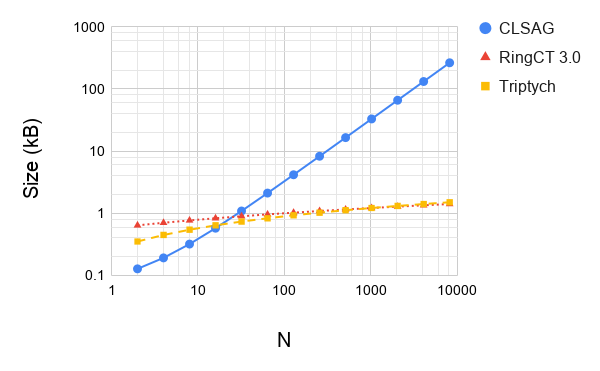
\includegraphics[width=0.6\textwidth]{size.png}
\caption{Proof sizes for input anonymity set size $N$}
\label{fig:size}
\end{figure}


\section{Future work}
It is possible to further extend the Triptych proving system to support proving knowledge of openings of multiple commitments within the \textit{same} anonymity set, while permitting the construction of linking tags for each such opening and demonstrating balance directly within a single proof.
Such a construction is much more efficient than the present work when built into a transaction protocol, but the security definitions applying to such a construction are still under evaluation.

\bibliographystyle{plain}
\bibliography{main}

\end{document}
